\documentclass{article}
\renewcommand{\familydefault}{\sfdefault}

\usepackage{geometry}
\usepackage{graphicx}
\usepackage{listings}
\usepackage{xcolor}

\geometry{margin=2cm}

\definecolor{brick-red}{RGB}{203,65,84}

\lstset{
    backgroundcolor=\color[gray]{0.95},
    basicstyle=\ttfamily\footnotesize,
    commentstyle=\color{brick-red},
    frame=single,
    framerule=0pt,
    framextopmargin=1em,
    framexbottommargin=1em,
    framexleftmargin=1em,
    framexrightmargin=1em,
    keepspaces=true,
    numbers=none,
    showstringspaces=false,
    xrightmargin=.05\textwidth,
    xleftmargin=.05\textwidth,
}

\title{Illumina vs. AVITI}

\author{thomas silvers}

\begin{document}

\maketitle

\noindent
We performed sequencing experiments on identical samples from the same donor (Baby 2, \texttt{B002}). In one experiment, Illumina was used; in the other, AVITI.

\section{Sequencing quality}

\section{Variant calling}

\section{Sequence typing}

We did sequence typing for E. coli (MLST name \texttt{Escherichia coli\#1}) using software \texttt{srst2} and with CLI pseudocode:

\begin{lstlisting}[language=bash]
srst2 --input_pe {trimmed reads} --mlst_* '{Escherichia_coli#1}'
\end{lstlisting}

\noindent
We found

\begin{itemize}
    \item \texttt{(ST)73} is the dominant type
    \item Results are nearly identical between platforms
    \item AVITI ($\times$) has higher depth at core genes used for typing
\end{itemize}

\begin{figure}[!h]
    \centering
    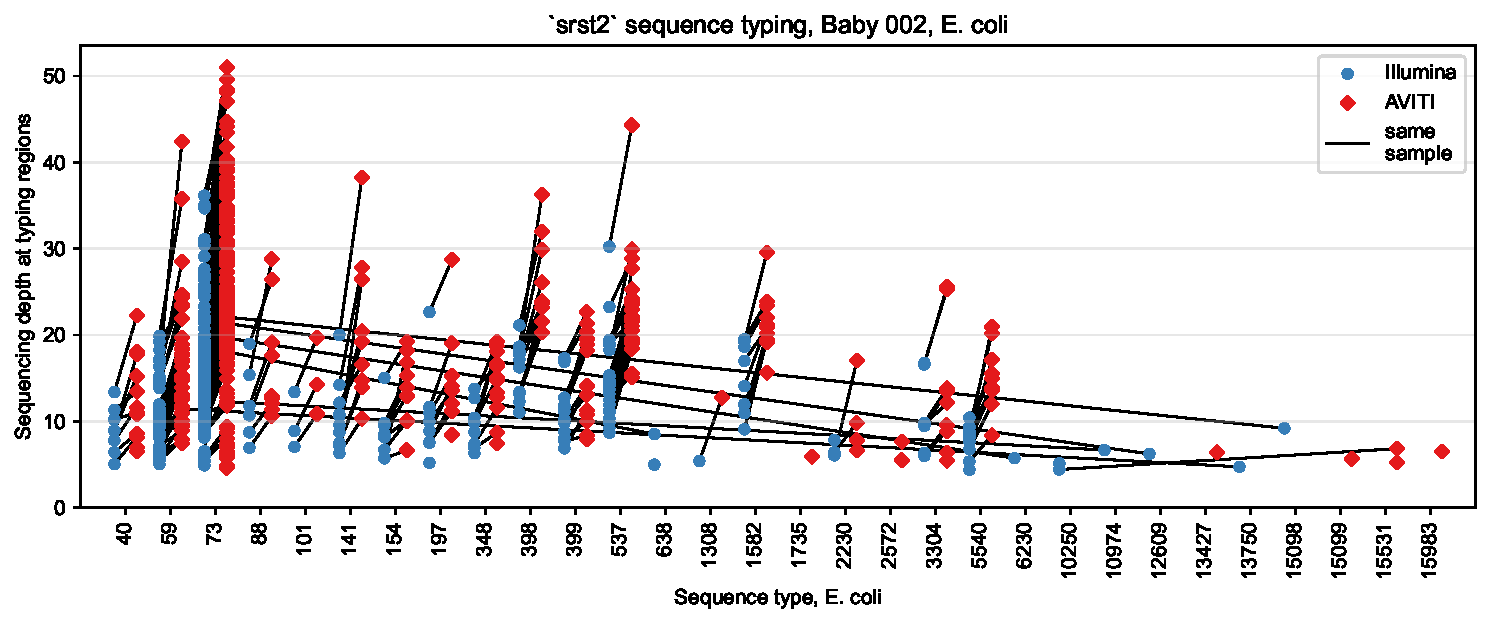
\includegraphics[width=.9\textwidth]{figures/sequence_typing.pdf}
    \label{fig:st}
\end{figure}

\section{Reconstructing phylogenies of dominant STs}

\section{Appendix}

Code to reproduce is available at \texttt{/raven/u/thosi/dev/projects/seqcomp}.

\end{document}